\begin{spacing}{1}
    \chapter*{Abstract}
\end{spacing}
Animotion is a combination of the two words animation and motion, cramming the general idea behind it into as little information as possible. This general idea being a camera, for example that of a laptop, a phone or an external one used in a computer setup, recording face and body gestures of the user and translating them onto a virtual reality model (VRM), thereby controlling it. This is done by using an artificial intelligence that calculates tracked gestures and puts them into a canvas that displays the default pose of the VRM and additional user input recorded by the camera. The aforementioned model can be selected by the user out of an assortment of three possible choices on the main page of the website. The moving VRM can be recorded, either by recording the browser window or the entire screen, and for example posted on social media for entertainment purposes. Another possible application would be using Animotion as a way of recording yourself for your own livestream (“V-Tubing”), where, for a variety of reasons, one chooses to not represent oneself with one’s own body but a virtual (“fictional”) one instead.
\\
The frontend, i.e., the website was mainly implemented using a combination of the JavaScript framework Next.js and Sass, a stylesheet language similar to CSS, or more accurately, an extension of it, used for the general design. For the web application MediaPipe, an open-source, cross-platform framework used to build machine learning solutions for streaming media, and Holistic, a gesture analysis and control library of MediaPipe that is mainly used for augmented reality effects, were chosen in order to depict the VRM together with three.js, a JavaScript library used to create and display 3D computer graphics in a web browser.
\\
\begin{figure}[htb]
    \centering
    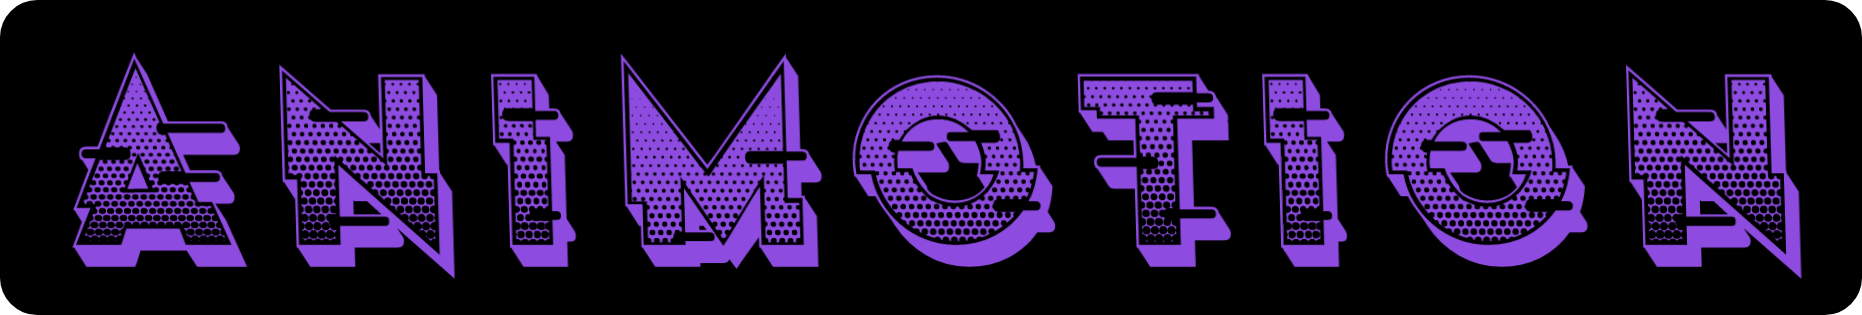
\includegraphics[width=0.8\textwidth]{pics/animotionlogo.png}
\end{figure}

\newpage
\begin{spacing}{1}
    \chapter*{Zusammenfassung}
\end{spacing}
Animotion ist eine Kombination aus den beiden Worten „Animation“ und „Motion“, wobei die generelle Idee dahinter in so wenig Information wie möglich zusammengefasst wird. Diese Idee ist, dass eine Kamera, zum Beispiel die eines Laptops, eines Handys oder eine externe Kamera in einem Computer-Setup, die Mimik und Gestik des Benutzers aufzeichnet und auf ein „Virtual Reality Model (VRM)“ überträgt, um es dadurch zu steuern. Dies wird durch eine künstliche Intelligenz erreicht, die verfolgte Gesten berechnet und sie auf eine Leinwand überträgt, die die Standardpose des VRM und zusätzliche, aufgenommene Benutzerbewegungen darstellt. Das eben erwähnte Modell kann aus einer Auswahl von drei möglichen Optionen auf der Hauptseite der Website selektiert werden. Das bewegende VRM kann aufgezeichnet werden, indem entweder das Browserfenster oder der gesamte Bildschirm aufgenommen wird, und zum Beispiel auf sozialen Medien zu Unterhaltungszwecken gepostet werden. Eine weitere mögliche Anwendung wäre die Verwendung von Animation zur Aufzeichnung von einem selbst für eine eigene Liveübertragung („V-Tubing“), bei der man aus verschiedenen Gründen sich selbst nicht mit dem eigenen Körper, sondern einem virtuellen („fiktionalen“) Körper darstellen möchte.
\\
Das Frontend, also die Website, wurde hauptsächlich mithilfe einer Kombination aus dem JavaScript-Framework Next.js und Sass, einer Stylesheet-Sprache ähnlich wie CSS, oder genauer gesagt eine Erweiterung, die für das allgemeine Design verwendet wird, implementiert. Für die Web-Anwendung wurden MediaPipe, ein open-source, plattformübergreifendes Framework, das zum Erstellen von Machine Learning-Lösungen für Übertragungsmedien verwendet wird, und Holistic, eine Gestenanalyse- und Steuerungsbibliothek von MediaPipe, die hauptsächlich für Erweiterte Realitätseffekte verwendet wird, ausgewählt, um das VRM zusammen mit three.js, einer JavaScript-Bibliothek, die verwendet wird, um 3D-Computergraphiken in einem Webbrowser anzuzeigen, darzustellen.
\\
\begin{figure}[htb]
    \centering
    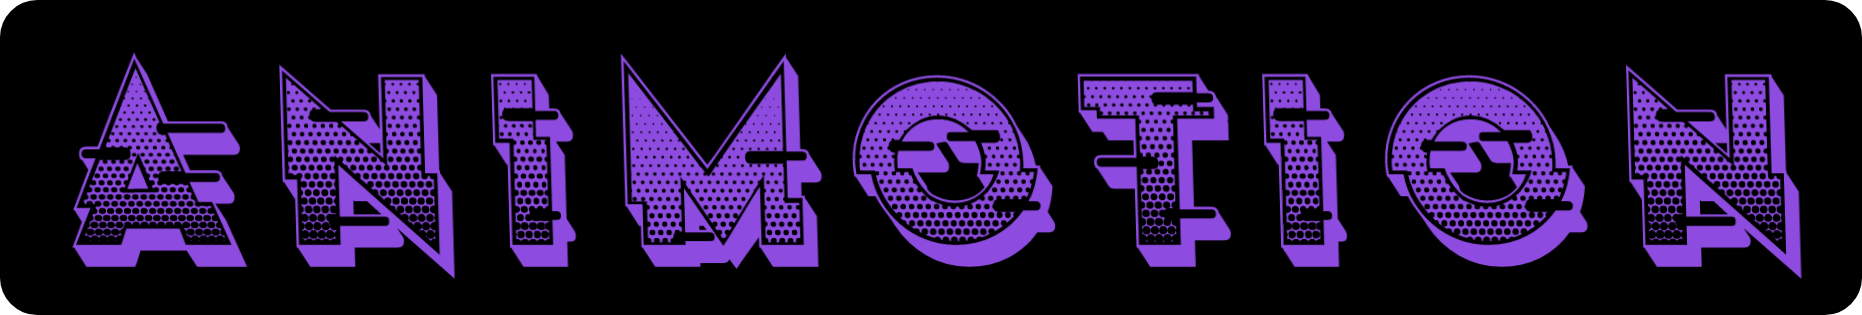
\includegraphics[width=0.1\textwidth]{pics/animotionlogo.png}
\end{figure}